
\subsection{MRI tank surface extraction}
The end tanks surfaces are very cruicial for estimating undistortion parameters. They will be used together 
with the CT tank measurements we obtained previously to do the estimation.

\subsection{extraction}
Comparing to CT images, MR images does not capture the materials of the phantom itself. It only captures 
signals generated from water and copper sulfate. However, depending on which secion of the phantom we are
looking at, there could be quite amount of noises that could be a challenge to remove. 

In the following sample MR image, we can see that top section's contrast ratio is pretty good. Not only that
we can easily identify it with our eyes, after slightly tweeking canny's algorithm, we can get a very good 
edge result. However, the bottom tank region is very noise. Although we can identify them our eye, canny
algorithm has a very hard time produce good edge result for that section. 

\begin{figure}[htb]
  \begin{minipage}[t]{2.75in}
    \centering
    \centerline{\mbox{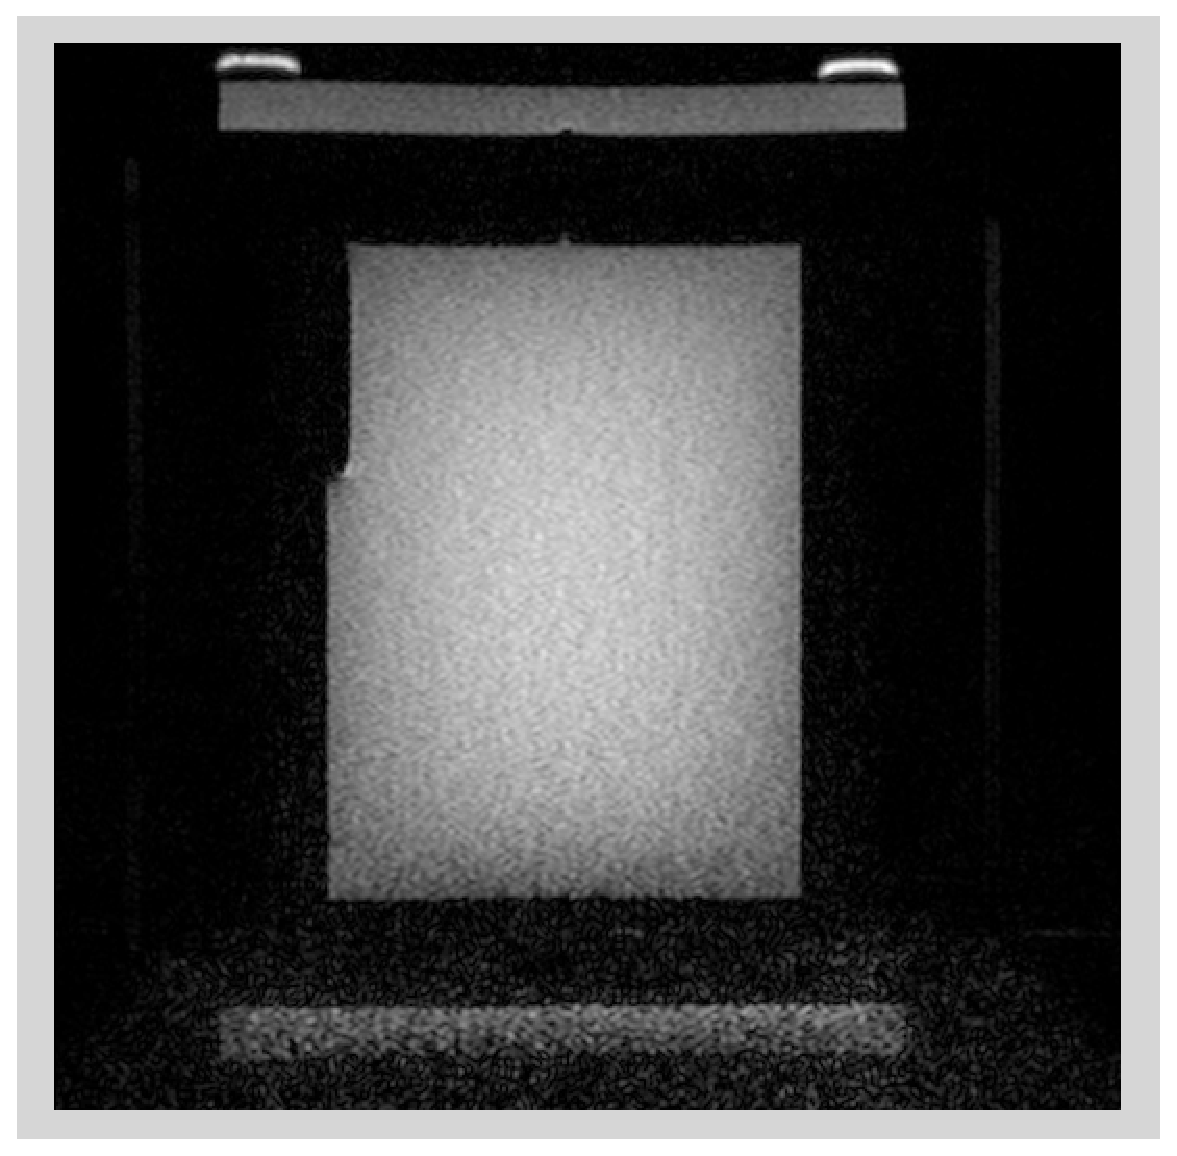
\includegraphics[width=2.75in]{data_extraction/images/MRI/mid_slice/112.eps}}}
    \centerline{\emph{(a) MR images}}
  \end{minipage}\medskip
  \begin{minipage}[t]{2.75in}
    \centering
    \centerline{\mbox{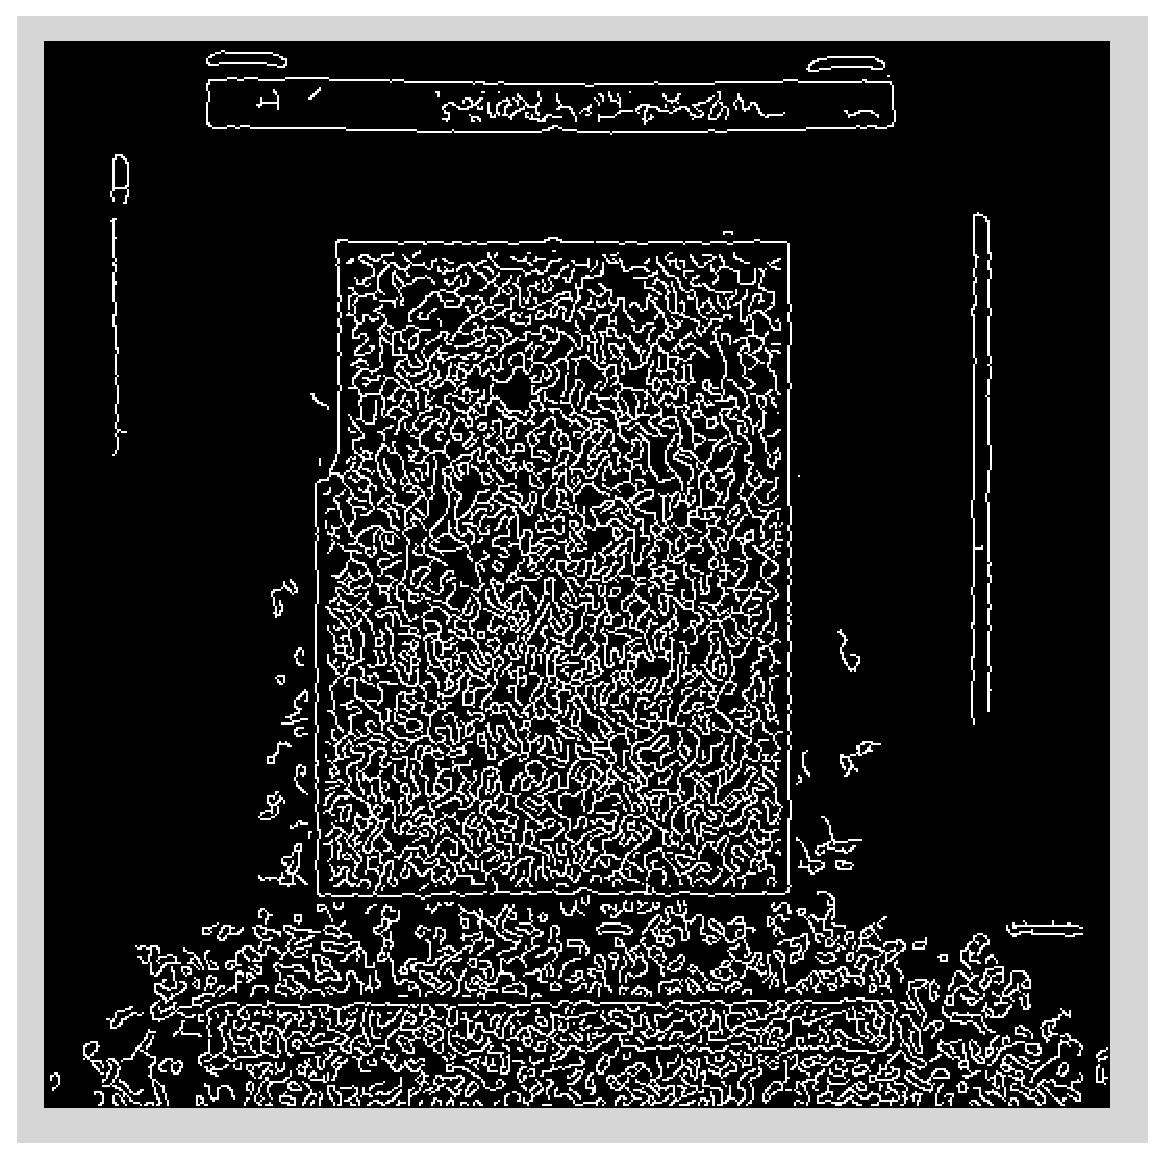
\includegraphics[width=2.75in]{data_extraction/images/MRI/mid_slice/112_canny_default.eps}}}
    \centerline{\emph{(b) Canny algorithm on (a) using default parameters}}
  \end{minipage}

  \begin{minipage}[t]{2.75in}
    \centering
    \centerline{\mbox{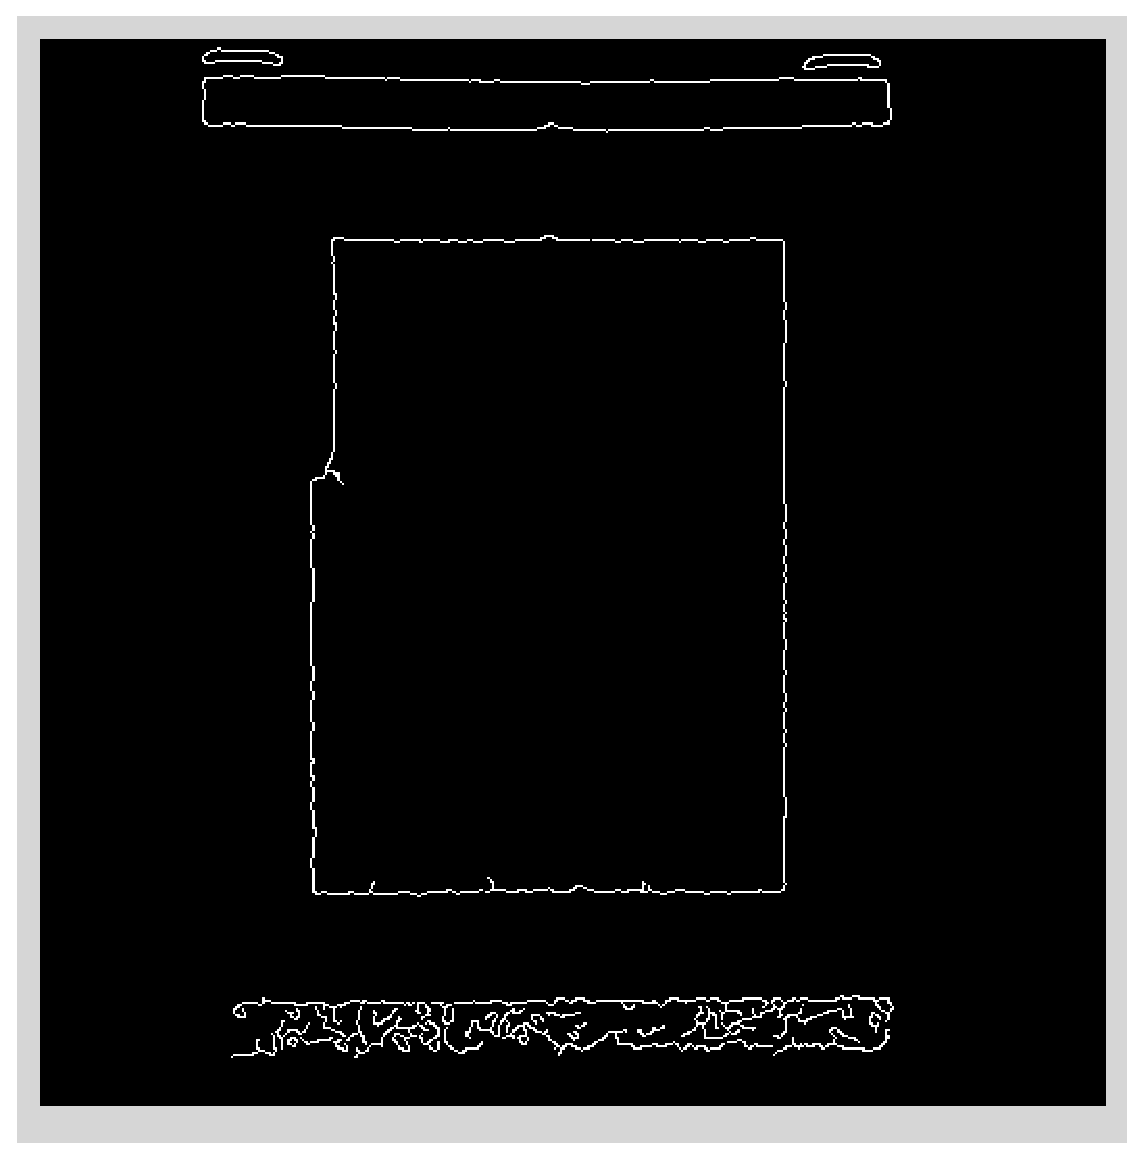
\includegraphics[width=2.75in]{data_extraction/images/MRI/mid_slice/112_canny_[0.1,0.2].eps}}}
    \centerline{\emph{(b) Canny algorithm on (a) using parameter [0.1, 0.2]}}
  \end{minipage}\medskip

  \begin{minipage}[t]{2.75in}
    \centering
    \centerline{\mbox{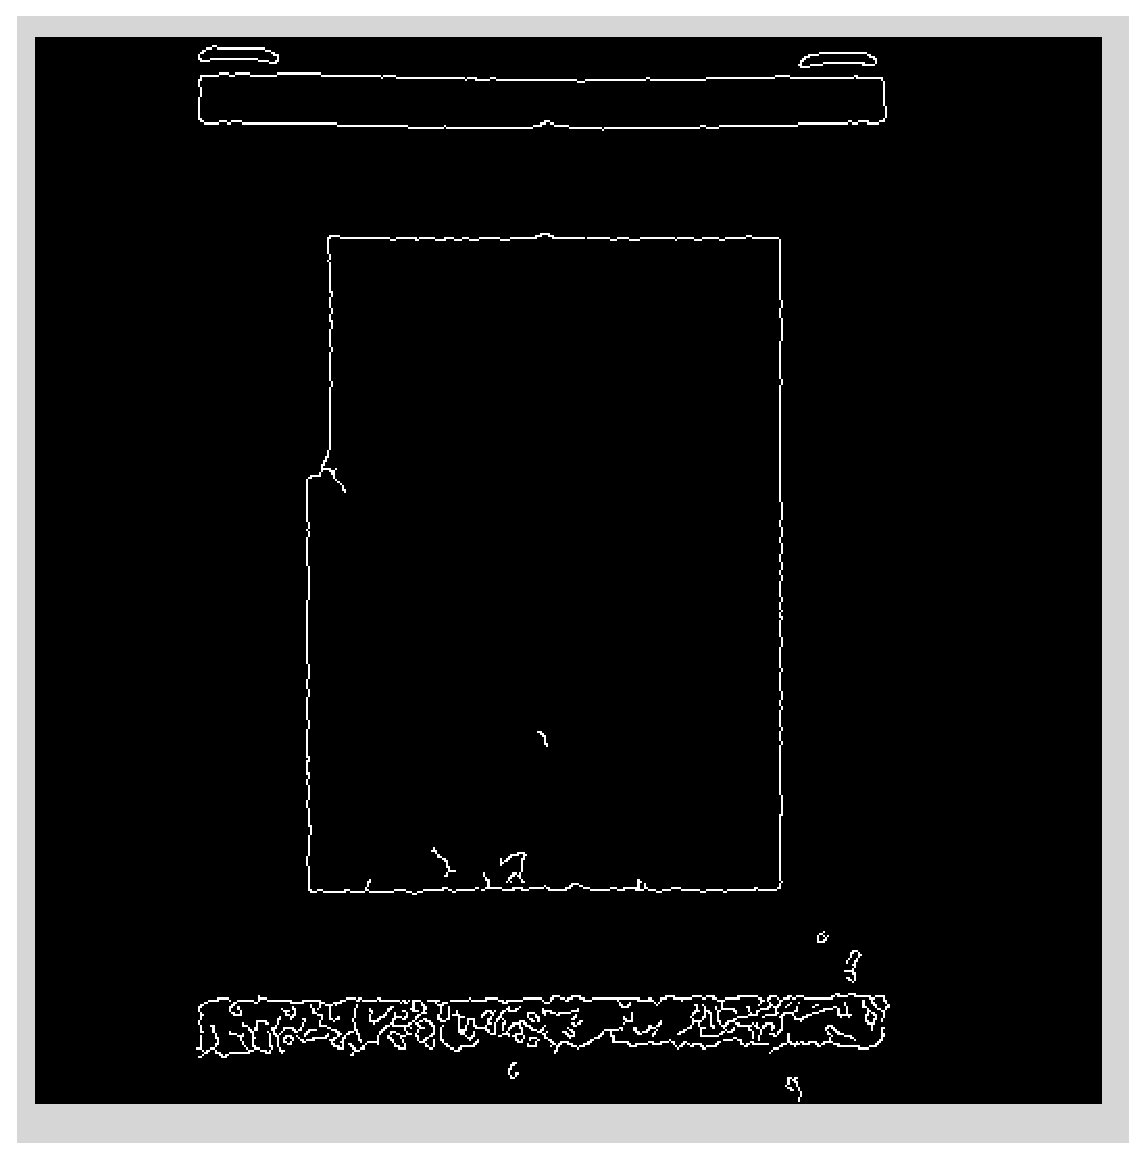
\includegraphics[width=2.75in]{data_extraction/images/MRI/mid_slice/112_canny_[0.09,0.18].eps}}}
    \centerline{\emph{(b) Canny algorithm on (a) using parameter [0.09, 0.18]}}
  \end{minipage}


\end{figure}


Since the overall layouts of tanks in MR images and CT images are quite similar -- they both have water tanks
at top and bottom of images and we are looking for top and bottom edges of those water tanks in both imagse.
So we decided that the best approach is to start with the algorithm we used in CT images even though there
are some big differences. Two big differences are:

\begin{enumerate}
  \item The surfaces we are looking for are curve due to distortion of the magnetic field.
  \item Water tanks appear in the bottom region of the images are quite noisy, by just tweeking canny's
    parameter will not give too much improvements.
\end{enumerate}

However, we believed that those issues could be overcome once we have reached the portion of algorithm that 
deal with those regions. On the bigger picture, we are still going to follow the same algorithm we used in
CT images water tank extractions:

\begin{enumerate}
  \item Use a middle slice to determine approximately where each surfaces are located, and we are going to
    used the same boundary to extract surface regions from every other images from the same image set. This 
    works because we have previously corrected any tiltness to each axis. So if a surface is in a particular
    region of one slice, we know for sure that it will be in the same region of other slices.
  \item Once we have extracted surface regions, we can determine the left and right boundaries of that surface
    by analysing the intensity histogram of each region.
  \item With each surface regions' left and right boundaries are set, we can apply our algorithms to filter out
    unwanted edges.
\end{enumerate}

\subsection{Region extraction}

One of the biggest challenge in dealing MR images is noise, especially the tank on the bottom of images. 
This water tank is sticking out of the head coil, so noises around that region is considerably larger than
other regions of the same image. Although canny algorithm does have a way to deal with noises in images by 
blurring source images, it is not enough to overcome the noises in MR images in order for us to get a very
good edge result.

Our approach is to sum previous and next slice of the imamge we are working on in order to cancel out some
noises and also enhance some features. Unlike CT images, in which flat surface will stay flat through out the
series. In MR images, due to the distortion of the magnetic field, flat surfaces will appear to be curved.
That curvature would get more and more severe toward the outer region of the phantom. This means when
overlapping previous and next images from the series to our target images, we could potentially add some 
pixels that does not belongs to the images we are processing. However, this is not a big issue for the
following reasons:

\begin{enumerate}
\item The overall distortion is quite small, the distorted outer edge of the water tank is approximately 
  3-4 pixels off the original position. This difference is spread out across 200 slices,
\item The reolution of the MR images is about 1mm, any changes smaller than 1mm won't get picked up. 
\end{enumerate}

So adding one slice before and one slice after will enhance the features we are looking for and will not 
add any unwanted features into the images.

Here is a comparison of the the histogram of before and middle column of middle slices before and after 
adding adjacent images.

% \begin{figure}[htb]
% \end{figure}

\subsection{Boundary detection}

For left and right boundary detection we are going to apply the similar method we used in CT images. 
Unlike CT images' left right boundaries, there is no phantom tank material signal in MR images, 
so we could just use maximum and minimum peak as a way to distinguish boundaries. Slices toward each end
of the phantom will have significantly more noises, they are very hard to distinguish. But if we use the same
method as we used in CT images we should have no problem detecting most boundaries which will give us more
than enough data for our estimation. This algorithm goes as follows:

\begin{enumerate}
  \item Run left-right boundary detection on the middle slice image. Due the good quality, we will get a 
    pretty accurate left and right boundary. The algorithm will not only return left and right boundary
    locations, but will also return several parameters used for tracking future boundaries.
  \item Run the algorithm two more passes, each run will take each half of the image set and iterate from
    the slice closest to mid slice to slice furthest to the mid slice. At the beginning of each run, we will
    pass the parameters we obtained from previous step.
  \item We just run this algorithm to the inside surface of exterior tank due to the fact that we had make
    sure there was no rotation and tiltness in each different axis. This means other three surfaces will
    share the left and right boundaries with exterior outside surface.
\end{enumerate}

\subsection{Noisy Edge reduction}

For noisy edge reduction, we are going to follow these steps:
\begin{enumerate}
  \item We are going to apply the short edges removal as we did in CT images. 
  \item After removing short edges, what's left are very hard to distinguish. In CT images, we knew the edges
    are supposed to be a straight line, so we filtered the noises based on a straight line model. In MR images,
    edges are distorted and are supposed to be curved. Since exterior tank gets very good signal and very good
    edge results, we can use the edge result from exterior tank's opposite surfaces' edge result as a model
    for filtering inferior tank's surface edge.
\end{enumerate}
